\section{Аналитический раздел}

\subsection{Анализ существующих решений}

По оценкам BusinesStat~\cite{businesstat}, начиная с 2020 года, основной тенденцией в сфере ветеринарных услуг России являются онлайн-консультации с ветеринарами. Также важно предоставлять клиенту информацию о его питомце и истории посещения клиники в электронном виде. Поэтому при анализе существующих решений были выделены следующие критерии:
\begin{enumerate}[label*=---]
	\item наличие мобильного приложения или сайта, через которое можно осуществлять действия в ветеринарной клинике;
	\item возможность ознакомиться с врачами и услугами клиники;
 	\item наличие личного кабинета для клиента с информацией о его питомцах;
 	\item возможность просмотра истории приемов.
 \end{enumerate}

Последние три критерия подразумевают действие через приложение или сайт, то есть онлайн.

\begin{table}[hbtp]
	\begin{center}
		\begin{flushleft}
			\captionsetup{justification=raggedright, singlelinecheck=false}
			\caption{\label{tab:solve}Сравнение существующих решений}
		\end{flushleft}
		\begin{tabular}{|  p{0.20\textwidth} | p{0.17\textwidth} | p{0.17\textwidth}  |  p{0.14\textwidth} | p{0.13\textwidth}|} 
			\hline  Существующее решение &Приложение/ сайт & Просмотр услуг  & Личный кабинет & История приемов \\ \hline
			
			petstroy~\cite{petstory} &   + &   + & + & - \\ \hline
			vet.city~\cite{vetcity} &   - &   - & - & +  \\ \hline
			vetcare24~\cite{vetcare24} &  - &  - & - & + \\ \hline
		\end{tabular}
	\end{center}
\end{table}

Из таблицы \ref{tab:solve} видно, что ни одно из существующих решений не удовлетворяет всем критериям.

\subsection{Формализация задачи}

В рамках курсовой работы необходимо спроектировать и разработать базу данных для ветеринарной клиники, а также приложение, позволяющее с ней работать. Разрабатываемое решение должно удовлетворять всем критериям, выдвинутым в предыдущем пункте. В ветеринарной клинике имеется разграничение по ролям: гость, авторизованный клиент, сотрудник клиники и администратор. Подробное описание их возможностей представлено на рисунке \ref{img:use-case}.

\begin{figure}[!h]
	\centering
	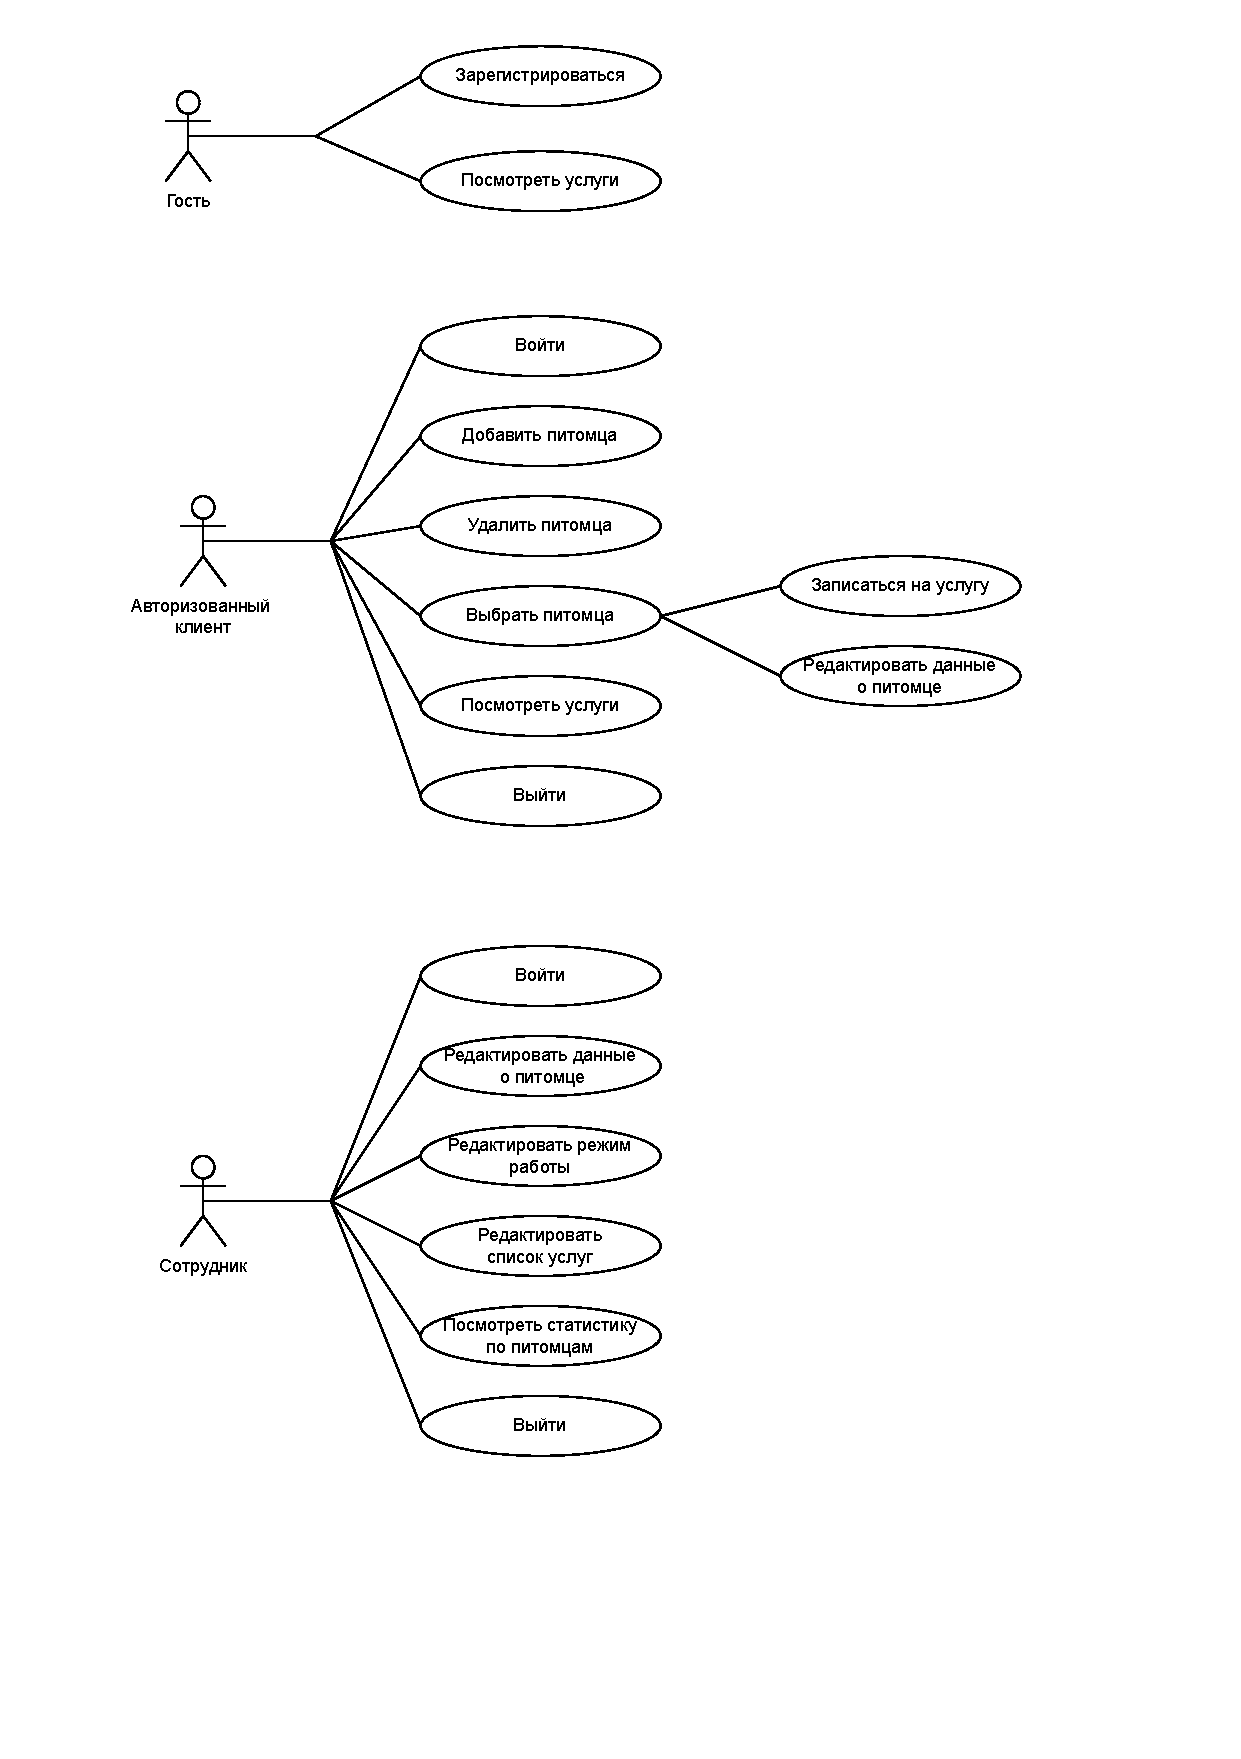
\includegraphics[width=\textwidth]{image/use-case.pdf}
	\caption{Диаграмма использования приложения}
	\label{img:use-case}
\end{figure}

\subsection{Формализация данных}

База данных должна хранить информацию о:
\begin{enumerate}[label*=---]
	\item пользователях с учетной записью (клиенты и работники);
	\item питомцах;
	\item записях на прием.
\end{enumerate}

ER-диаграмма сущностей в нотации Чена, описывающая сущности, их атрибуты и связи между сущностями в разрабатываемой базе данных, представлена на рисунке \ref{img:er}.

\begin{figure}[!h!]
	\centering
	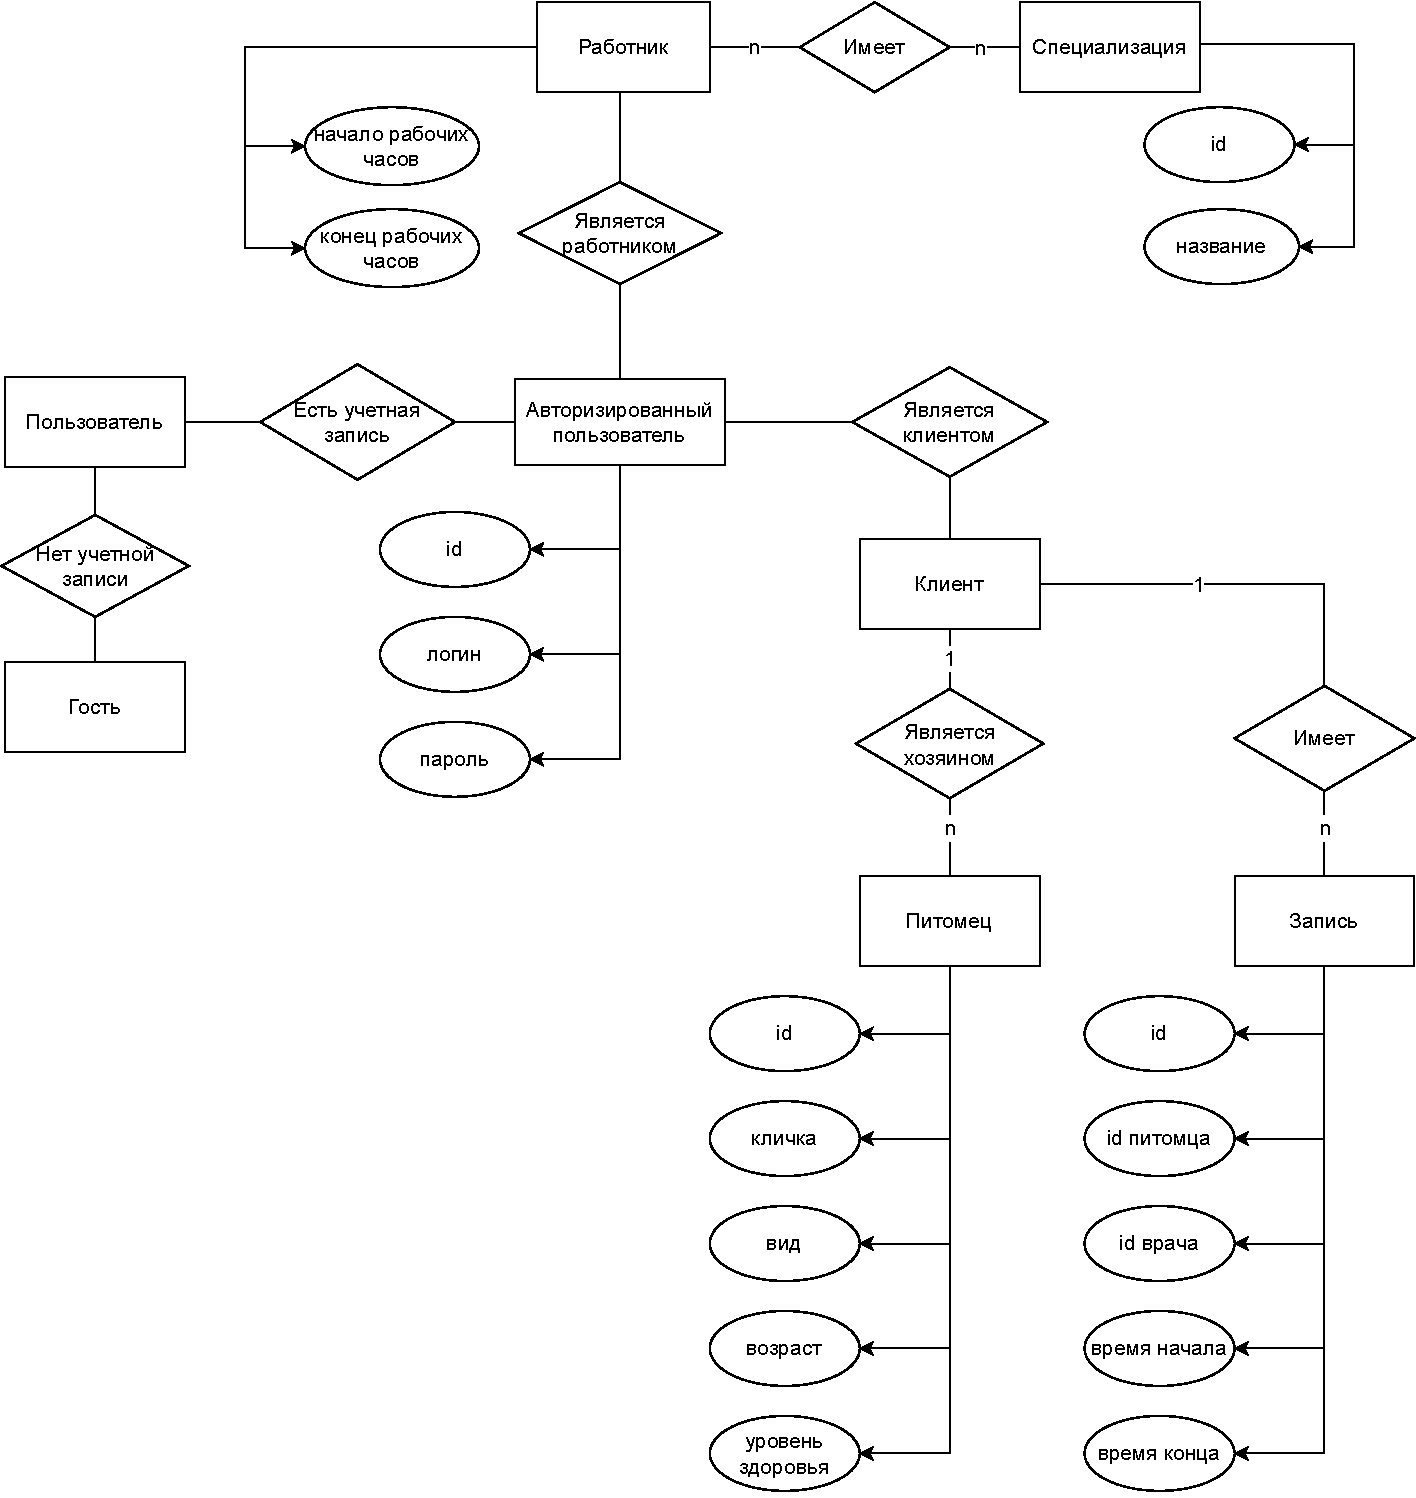
\includegraphics[width=165mm]{image/er.pdf}
	\caption{ER-модель в нотации Чена}
	\label{img:er}
\end{figure}
\newpage

\subsection{Анализ базы данных и системы управления базами данных}

По модели хранения базы данных делятся на три группы: дореляционные, реляционные и постреляционные~\cite{Date}. 

\subsubsection{Дореляционные базы данных}

К дореляционным базам данных относятся:

\begin{enumerate}[label*=---]
	\item инвертированные списки;
	\item иерархичекие;
	\item сетевые.
\end{enumerate}

База данных на основе инвертированных списков представляет собой совокупность файлов, содержащих записи. Для записей в файле определен некоторый порядок, диктуемый физической организацией данных. Для каждого файла может быть определено произвольное число других упорядочений на основании значений некоторых инвертированных списков. 

Иерархическая модель  состоит из объектов с указателями от родителей к потомкам, соединяя вместе связанную информацию. Такие базы данных могут быть представлены как дерево.

К основным понятиям сетевой модели относятся: элемент (узел), связь. Узел -- это совокупность атрибутов данных, описывающих некоторый объект. Сетевая модель не является полностью независимой от приложения, так как выборка данных зависит от физической организации хранилища. Другими словами, если необходимо изменить структуру данных, то нужно поменять и приложение~\cite{Begg}.

\subsubsection{Реляционные базы данных}

Реляционные базы данных чаще используют язык SQL~\cite{oracle}. Данные реляционных баз хранятся в виде таблиц и строк, таблицы могут иметь связи с другими таблицами через внешние ключи, таким образом образуя отношения~\cite{sql}. 

Структура таких баз данных позволяет связывать информацию из разных таблиц с помощью внешних ключей (или индексов), которые используются для уникальной идентификации любого атомарного фрагмента данных в этой таблице. Другие таблицы могут ссылаться на этот внешний ключ, чтобы создать связь между частями данных и частью, на которую указывает внешний ключ. Важным свойством реляционных баз данных является их способность удовлетворять требованиям ACID~\cite{acid}:~атомарность,~согласованность,~изоляция,~устойчивость.

 
\subsubsection{Постреляционные базы данных}

Постреляционная модель данных является расширенной реляционной моделью, которая снимает ограничение неделимости хранящихся в записях таблиц данных. В таких базах данных реализована работа со сложными типами данных, создаваемых пользователями. Такие решения не всегда могут обеспечить полную поддержку ACID. 

Нереляционные хранилища можно использовать вместе с реляционными базами данных. Например, в системах, где основной объем информации хранит SQL, а за кэш отвечает нереляционная база данных~\cite{amazon}.

\subsection*{Вывод}

С учетом особенности задачи была выбрана реляционная модель хранения данных, так как предметная область может быть представлена в виде <<таблиц>> и должна удовлетворять требованиям ACID. В качестве системы управления базой данных в данной работе будет использоваться PostgreSQL~\cite{postgres}.
